\documentclass[10pt]{article}

%% Various useful packages and commands from different sources

\usepackage[applemac]{inputenc}
\usepackage[english]{babel}
\usepackage[T1]{fontenc}
\usepackage{cite, url,color} % Citation numbers being automatically sorted and properly "compressed/ranged".
%\usepackage{pgfplots}
\usepackage{graphics,amsfonts}
\usepackage[pdftex]{graphicx}
\usepackage[cmex10]{amsmath}
% Also, note that the amsmath package sets \interdisplaylinepenalty to 10000
% thus preventing page breaks from occurring within multiline equations. Use:
 \interdisplaylinepenalty=2500
% after loading amsmath to restore such page breaks as IEEEtran.cls normally does.

% Compact lists
\usepackage{enumitem}
\usepackage{booktabs}
\usepackage{fancyvrb}

\usepackage{listings} % for Matlab code
\definecolor{commenti}{rgb}{0.13,0.55,0.13}
\definecolor{stringhe}{rgb}{0.63,0.125,0.94}
\lstloadlanguages{Matlab}
\lstset{% general command to set parameter(s)
framexleftmargin=0mm,
frame=single,
keywordstyle = \color{blue},% blue keywords
identifierstyle =, % nothing happens
commentstyle = \color{commenti}, % comments
stringstyle = \ttfamily \color{stringhe}, % typewriter type for strings
showstringspaces = false, % no special string spaces
emph = {for, if, then, else, end},
emphstyle = \color{blue},
firstnumber = 1,
numbers =right, %  show number_line
numberstyle = \tiny, % style of number_line
stepnumber = 5, % one number_line after stepnumber
numbersep = 5pt,
language = {Matlab},
extendedchars = true,
breaklines = true,
breakautoindent = true,
breakindent = 30pt,
basicstyle=\footnotesize\ttfamily
}

\usepackage{array}
% http://www.ctan.org/tex-archive/macros/latex/required/tools/
\usepackage{mdwmath}
\usepackage{mdwtab}
%mdwtab.sty	-- A complete ground-up rewrite of LaTeX's `tabular' and  `array' environments.  Has lots of advantages over
%		   the standard version, and over the version in `array.sty'.
% *** SUBFIGURE PACKAGES ***
\usepackage[tight,footnotesize]{subfigure}
\usepackage[top=2.2cm, bottom=2.2cm, right=1.7cm,left=1.7cm]{geometry}
\usepackage{indentfirst}


%\setlength\parindent{0pt}
\linespread{1}

\usepackage{mathtools}
\DeclarePairedDelimiter{\ceil}{\lceil}{\rceil}
\DeclarePairedDelimiter{\floor}{\lfloor}{\rfloor}
\DeclareMathOperator*{\argmax}{arg\,max}
\newcommand{\M} {\mathtt{M}}
\newcommand{\dB} {\mathrm{dB}}
\newcommand{\tr} {\mathrm{tr}}



\graphicspath{ {figures/} }

% equations are numbered section by section
%\numberwithin{equation}{section}


\begin{document}
\title{Digital Transmission - Homework 2}
\author{Andrea Dittadi, Davide Magrin, Michele Polese}

\maketitle

\section*{Problem 1}

\subsection*{Choice of $N_h$}

In order to determine a suitable $N_h$ (i.e., the number of rays of the impulse response we will keep), we consider the noise that we would introduce by performing the truncation of the power delay profile \textit{PDP} (that corresponds to a truncation of the number of rays of the channel impulse response). The aleatory part of the discrete power delay profile of the channel is given as the sampled version of
\begin{equation}
\M(\tau) = \frac{1}{\bar{\tau}_{rms}} e^{-\tau / \bar{\tau}_{rms}}
\end{equation}
that is
\begin{equation}
\M(iT_C) = \frac{1}{\bar{\tau}_{rms}} e^{-iT_C / \bar{\tau}_{rms}}
\end{equation}
with $i$ non-negative integer, $\tau_{rms} = 0.3T$ the average rms delay spread and $T_C = 1 = T/4$. This quantity must be then normalized in such a way that
\begin{equation}
\sum_{i=0}^{\infty} \M(iT_C) = 1 - C^2
\end{equation}
where $C = \sqrt{K / (K+1)}$ is the deterministic line of sight (\textit{LOS}) component of the first ray (for $i=0$) and $K$ is the provided Rice factor. In order to compute the infinite sum above, only the initial 895 samples are actually used, as MATLAB approximates all $\M(iT_C)$ values for $i > 895$ to zero.

Knowing that the true impulse response of the channel has random properties described by the power delay profile $\M(iT_C)$ and by the quantity $C$, then we define the quality of the approximation due to truncation as
\begin{equation}
\Lambda_t(N_h) = \frac{E[||\mathbf{h}||^2]}{E[||\mathbf{\Delta h}||^2]} = \frac{C^2 + \sum_{i=0}^{\infty} \M(iT_C)}{\sum_{i=N_h}^{\infty} \M(iT_C)}
\end{equation}
where $\mathbf{h}$ is the vector of the impulse response $[h_0(nT_C),~h_1(nT_C),\ldots]$ and therefore
\begin{equation}
E[||\mathbf{h}||^2] = E[\sum_{i=0}^{\infty} |h_i(nT_C)|^2] = C^2 + \sum_{i=0}^{\infty} \M(iT_C).
\end{equation}
The noise in the system is
\begin{equation}
\Lambda = \frac{\M_x E[||\mathbf{h}||^2]}{4 \sigma_w^2} = \frac{\M_x (C^2 + \sum_{i=0}^{\infty} \M(iT_C))}{4 \sigma_w^2}
\end{equation}
where $\M_x$ is the statistical power of the input signal. Finally, we define the normalized ratio
\begin{equation}
\Lambda_n (N_h) = \frac{\Lambda_t}{\Lambda} = \frac{4 \sigma_w^2}{\M_x \sum_{i=N_h}^{\infty} \M(iT_C)}
\end{equation}
to compare the noise of the system with the noise we are introducing by truncating $\M(iT_C)$ to $N_h$ samples.

Looking at the plot of $\Lambda_n (N_h)_{\dB}$ against $N_h$ in Fig.~\ref{fig:p01_lambda_n}, we can maintain that $N_h = 3$ is a good choice, since we have $\Lambda_n(2) \approx 2~\dB$ and $\Lambda_n(3) \approx 5.6~\dB$.

\begin{figure}[ht]
	\centering
	\includegraphics[width=0.52\textwidth]{p01_lambda_n}
	\caption{Plot of $\Lambda_n (N_h)$ in dB for the choice of $N_h$.}
    \label{fig:p01_lambda_n}
\end{figure}

\subsection*{Determine $E[|h_i(nT_C)|^2]$}
Given $N_h = 3$, the PDP of the channel $E[|h_i(nT_C)|^2], i = 0, 1, 2$ in $\dB$ is reported in Fig.~\ref{fig:pdp} and in Table~\ref{table:pdp}. Note that this power delay profile includes the power of aleatory $\tilde{h}_i(nT_C)$ components and the deterministic LOS component added on ray $i = 0$.

\begin{table}[h!]
  \centering
  \begin{tabular}{c|c|c|c}
    $ i $ & $ 0 $ & $ 1 $ & $ 2 $ \\ \hline
    $E[|h_i(nT_C)|^2]$ [$\dB$] & -0.596 & -10.488 & -14.107
  \end{tabular}
  \caption{$E[|h_i(nT_C)|^2], i = 0, \dots, N_h-1$ in $\dB$ (PDP)}
  \label{table:pdp}
\end{table}

\begin{figure}[h!]
  \centering
  \includegraphics[width = 0.6\textwidth]{p01_pdp}
  \caption{Plot of the values $E[|h_i(nT_C)|^2]$ [$\dB$] of PDP for each ray $ i \in [0,2]$}
  \label{fig:pdp}
\end{figure}

\subsection*{Channel simulation}
In order to generate the impulse response of the channel we used the model proposed in \cite{bc} and reported in Fig.~\ref{fig:chimp}.
\begin{figure}[h!]
  \centering
  \includegraphics[width = 0.7\textwidth]{p01_channelmodel}
  \caption{Model used to simulate the channel impulse response}
  \label{fig:chimp}
\end{figure}

For each ray $i = 0, 1, \dots, N_h -1$ the system is fed with $w_i(lT_p)$, which is complex white noise with zero mean and unit power, generated with the MATLAB function \texttt{wgn}. This signal is filtered with a narrowband shaping filter in order to impose the shape of classical Doppler spectrum
\begin{equation}
  \mathcal{D}(f) =  \begin{cases} \frac{1}{\pi f_d} \frac{1}{\sqrt{1-(f/f_d)^2}}, & |f| \le f_d \\
                                  0                                              & \mbox{otherwise}
                   \end{cases}
\end{equation}
The filter $h_{ds}$ is such that $|\mathcal{H}_{ds}|^2 = \mathcal{D}(f)$. Since the Doppler spread $f_d = 5*10^{-3}\frac{1}{T} = 5*10^{-3}\frac{1}{4T_C}$ is very close to DC it is an hard task to design a digital lowpass filter that approximate the desired function while working with $T_C$ as the sampling period. Therefore it is necessary to generate the white noise $w_i(lT_p)$ and filter it using a different sampling period $T_p = Q_{int}T_C$. In particular, in order to use the filter designed in \cite{anachugg}, let $T_p f_d = 0.1$ thus $T_p = 0.1 \frac{4 T_C}{5*10^{-3}} = 80 T_C$.

This filter is an IIR narrowband filter which is the convolution of a filter that approximates the classical Doppler spectrum for $f \le f_d$ and of a Chebychev lowpass filter with cutoff frequency $f_d$. Since $h_{ds}$ is an IIR filter the effect of transient on the filtered signal is potentially infinite, however the impulse response of $h_{ds}$ is approximated to zero by MATLAB for $i > 282$. Therefore to discard the transient effect at the output of the scheme in Fig.~\ref{fig:chimp} the simulator drops $282*Q_{int}$ samples. This is a conservative choice: in order to keep the noise generated by truncation of IIR impulse response below system noise less than 282 coefficients would be enough. However, since the generation of the impulse response of radio channel is performed offline and there aren't memory or computational constraints we stick to this choice. The filter is normalized by its energy $E_{h_{ds}} = \sum_{i = 0}^{\infty} h_{ds} (iT_p) \approx \sum_{i = 0}^{282} h_{ds} (iT_p)$.

The interpolator filter $h_{int}$ performs interpolation using the spline algorithm, then each impulse response $h'_i(kT_C)$ is multiplied by $\sigma_i = \sqrt{E[|\tilde{h}_i(nT_C)|^2]}$ in order to apply the desired power delay profile. Note that $E[|\tilde{h}_i(nT_C)|^2], i = 0, \dots, N_h -1$ is the PDP obtained by sampling the continuous $M(\tau)$ PDP and normalizing it to $1-C^2$, thus it describes the power of the aleatory component of each ray. Finally, for the ray $i = 0$ the LOS component $C$ is added.

This procedure is repeated for each ray $i = 0, 1, 2$ and the generated impulse response $h_i(nT_C)$ is stored without the transient in the $i$-th row of the matrix \texttt{h\_mat}. As a matter of fact, the simulation requires on average 6 ms for the generation of transient samples and 0.35 s for the generation of $2*10^6$ useful samples, therefore even with a conservative choice for the transient its computation requires about $1.7\%$ of the whole simulation time.


\subsection*{Show the behavior of $|h_1(nT_C)|$}
The behavior of $|h_1(nT_C)|, n = 0, 1, \dots, 1999$ can be observed in Fig.~\ref{fig:h1}.

\begin{figure}[h!]
  \centering
  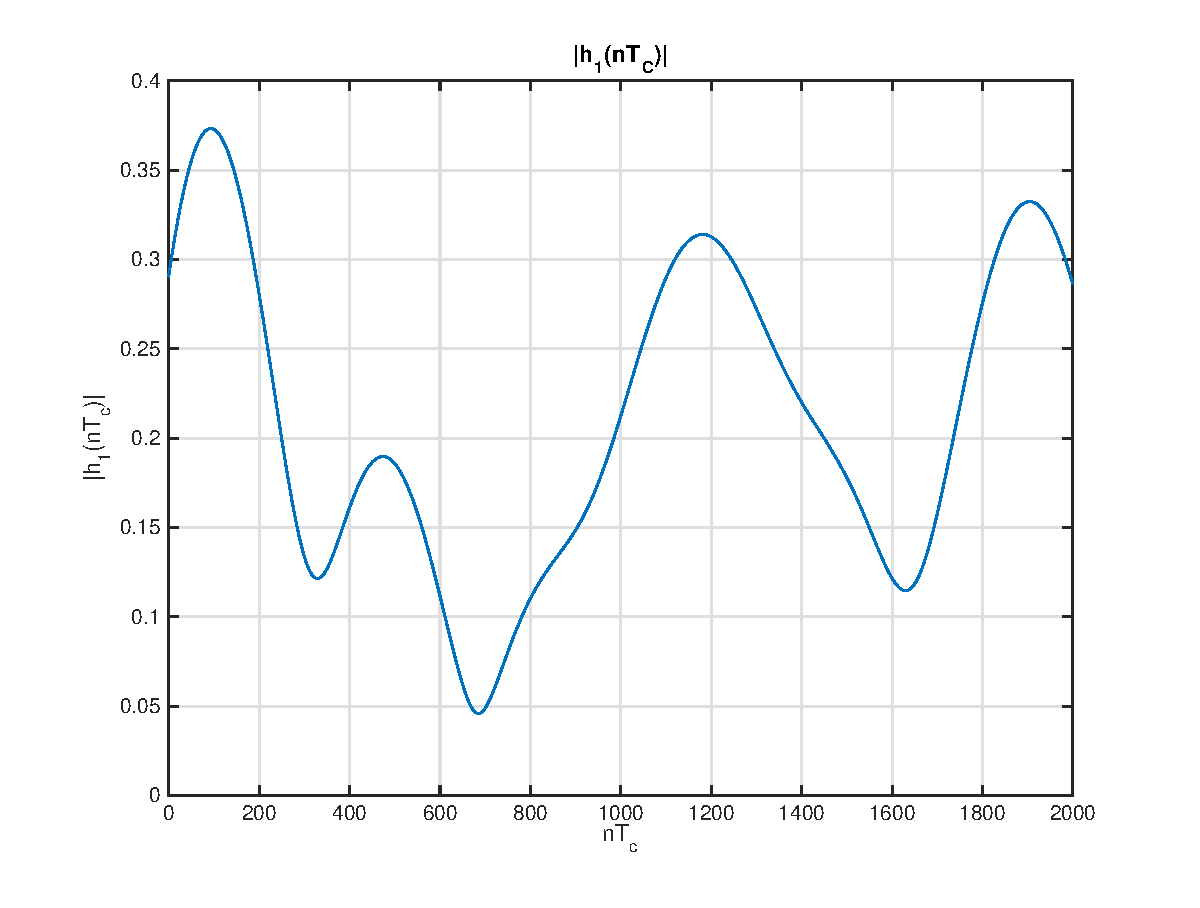
\includegraphics[width = 0.6\textwidth]{p01_h1}
  \caption{$|h_1(nT_C)|, n = 0, 1, \dots, 1999$}
  \label{fig:h1}
\end{figure}

\subsection*{Plot the histogram of $\frac{|h_1|}{\sqrt{E[|h_1|^2]}}$}
Since $\frac{|h_1|}{\sqrt{E[|h_1|^2]}}$ is the scaled absolute value of a complex gaussian random variable, it is distributed according to a Rayleigh distribution with PDF
$$p_{|\bar{g}_i|}(a) = 2a e^{-a^2} 1(a)$$

The histogram of $\frac{h_1}{\sqrt{E[|h_1|^2]}}$, computed over a window of 1000 samples of a single realization of the channel's impulse response, is shown in Fig.~\ref{fig:h1hist}. We can observe that the empirical pdf does not approximate the Rayleigh distribution. Indeed, as Fig.~\ref{fig:h1histvstime} shows, whenever $h_1$ shows a local maximum or minimum, the values for consecutive time instants are similar, therefore they build up in the histogram to create peaks. In order to explain this behavior let's consider the coherence time of the channel. This is a parameter defined as the inverse of the Doppler spread $f_d$, therefore $T_{coh} = 1/f_d = \frac{T}{5*10^{-3}}$ but since the channel is defined in the time domain $T_C = T/4$ the coherence time with respect to the channel sampling time actually is $T_{coh} = 1/f_d = \frac{4T_C}{5*10^{-3}} \approx 833T_C$.
The coherence time is the range over which the autocorrelation of the impulse response of ray $h_1$ is approximately non zero. Therefore, two samples of $h_1$ at a lag less than $T_{coh}$ are correlated and not statistically independent, even though drawn from the same distribution. Since the interval of 1000 consecutive samples over which the histogram is evaluated contains just one coherence interval and thus correlated samples, it is not representative of the complete distribution of $h_1$ values. On the other hand, if we increase the window of observed samples to (TODO) value, it can ben seen that the histogram approaches the expected Rayleigh distribution, since the number of independent samples observed grows. The histogram is an estimator of the probability density function, which is the derivative of the CDF. According to Glivenko-Cantelli theorem (TODO needs citation), the empirical CDF computed as $\hat{F}_n(x) = \frac{1}{x}\sum_{i = 0}^n \texttt{I}_x(i)$, with $\texttt{I}_x(i)$ the indicator function, converges to the real CDF as the number of independent observations of the process grows.
% TODO Also include pics of hist getting better with more samples or it didn't happen

\begin{figure}[h!]
  \centering
  \includegraphics[width = 0.6\textwidth]{p01_h1hist}
  \caption{Histogram of $\frac{h_1(nT_C)}{\sqrt{E[|h_1|^2]}}, n = 0, 1, \dots, 999$}
  \label{fig:h1hist}
\end{figure}

\begin{figure}[h!]
  \centering
  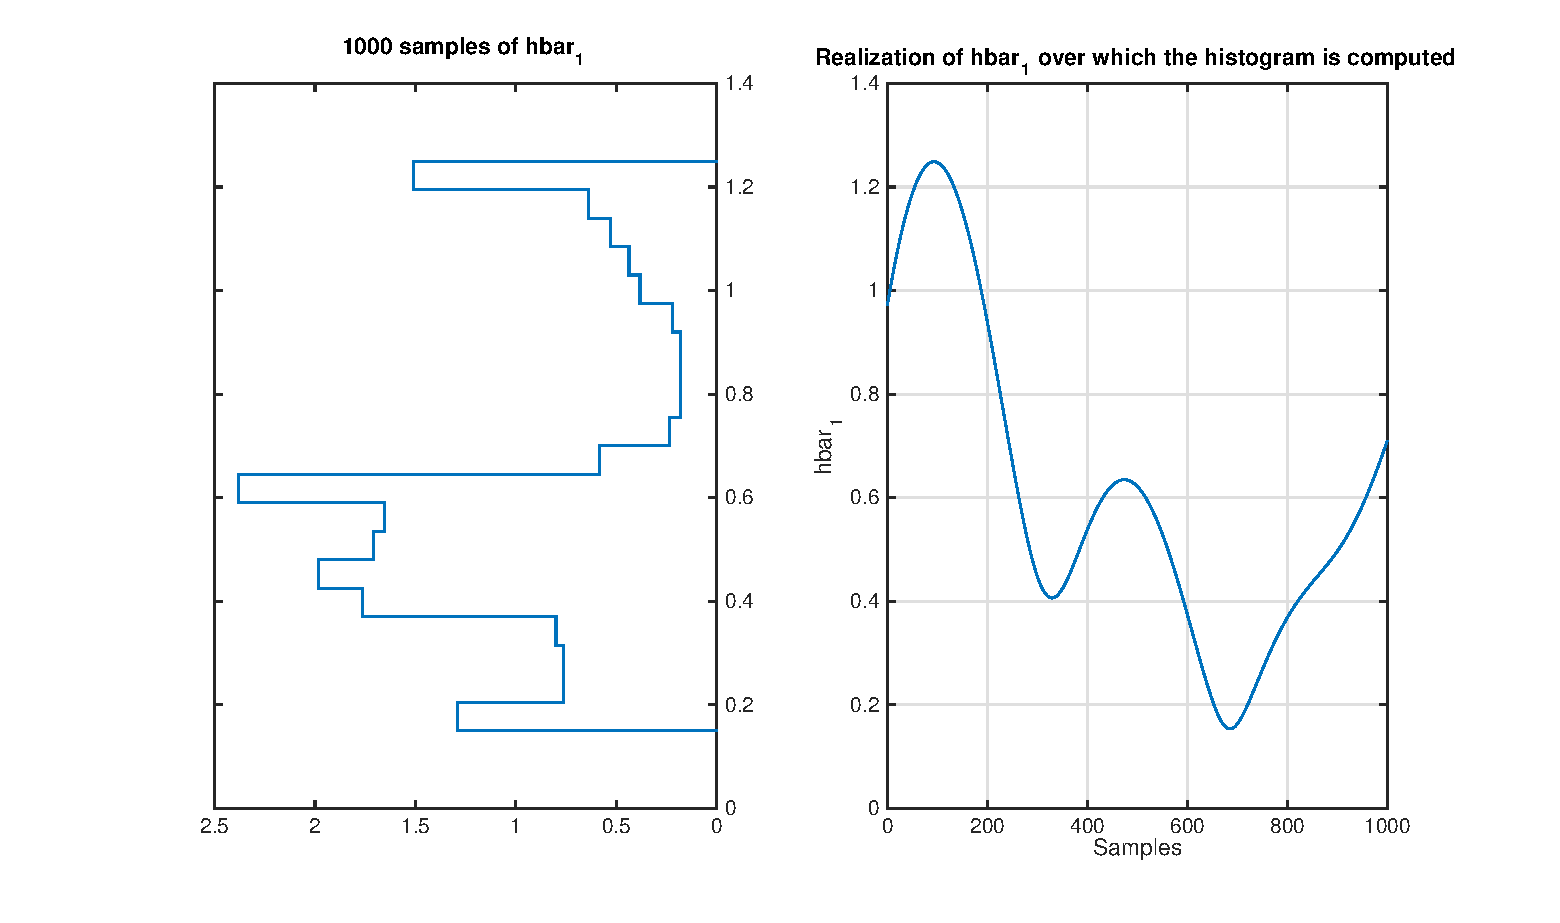
\includegraphics[width = 0.8\textwidth]{p02_h1hist}
  \caption{Comparison between the histogram and the time domain data it was derived from}
  \label{fig:h1histvstime}
\end{figure}

\subsection*{Plot the histogram of $\frac{|h_1(151T_C)|}{\sqrt{E[|h_1(151T_C)|^2]}}$ for 1000 realizations}
In this section we adopt a different approach to study the distribution of the values of $h_1$ and study the values that the same sample $\frac{|h_1(151T_C)|}{\sqrt{E[|h_1(151T_C)|^2]}}$ assumes over 1000 different realizations of the channel. The histogram that this simualtion generates can be seen in Fig.~\ref{fig:h1hist1000realizations}. As it can be seen, it approximates the Rayleigh distribution $p_{|\bar{g}_i|}(a) = 2a e^{-a^2} 1(a)$ in a better way than Fig. \ref{fig:h1hist}, since in this case the samples that are considered when computing the histogram are drawn from independent realizations of the process. Note that $E[|h_1(151T_C)|^2]$ is actually equal to the value of the PDP for ray $i=1$.

\begin{figure}[h!]
  \centering
  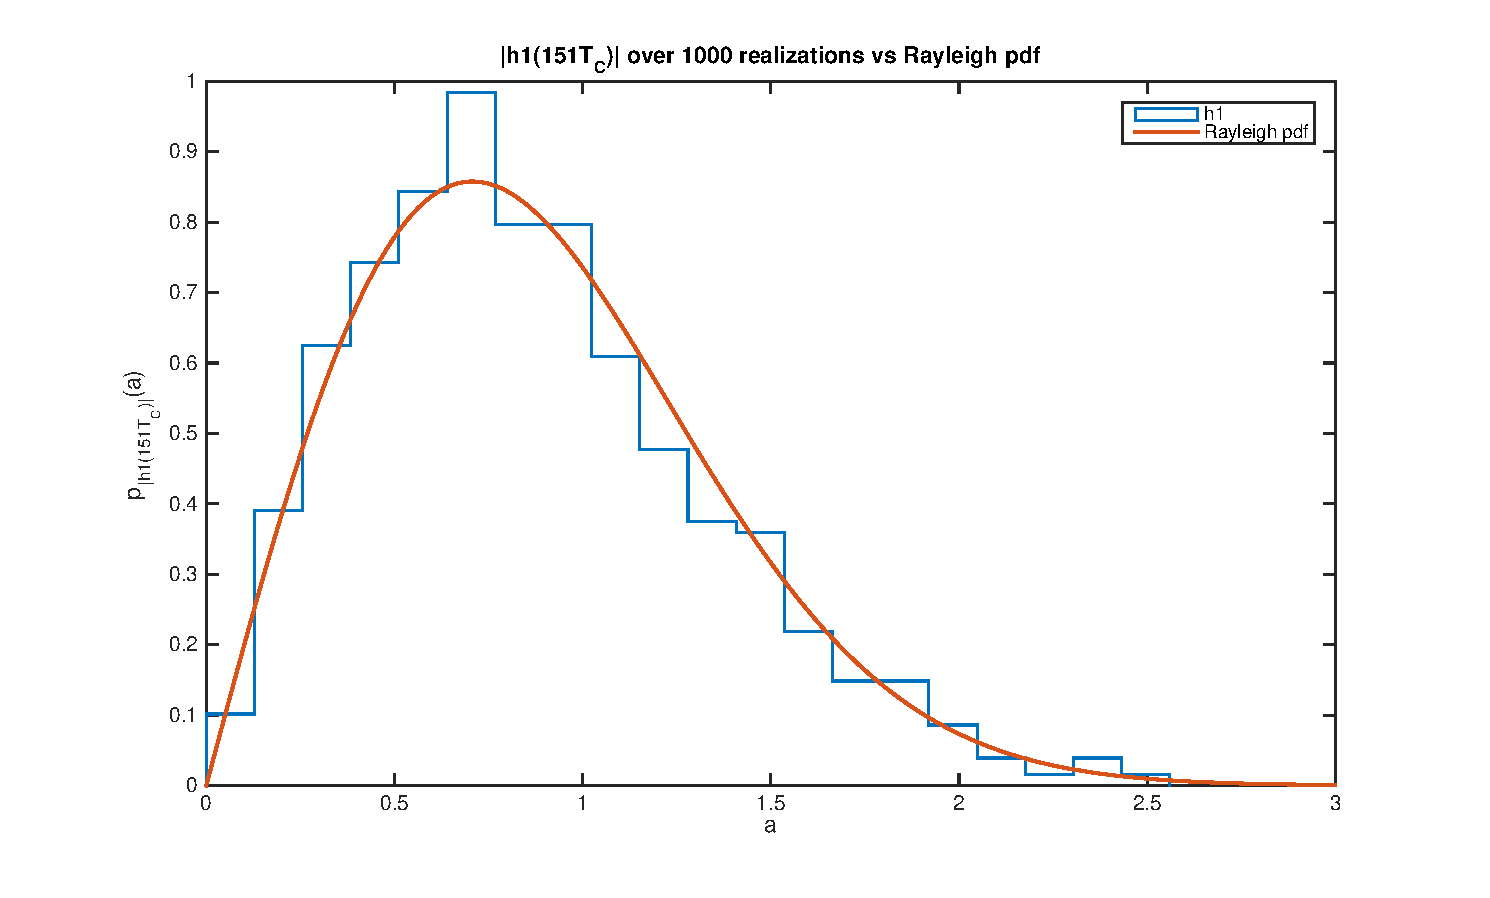
\includegraphics[width = 0.8\textwidth]{p03_h1hist}
  \caption{Histogram of a single sample of $h_1$ across different realizations vs the expected Rayleigh pdf}
  \label{fig:h1hist1000realizations}
\end{figure}

\clearpage

\section*{Problem 2}

\subsection*{Setup of the receiver}
% TODO Draw the polyphase implementation of the channel. This will help clarify what $N_i$ and $N$ are.

The channel can be simulated using the model depicted in Fig.~\ref{fig:channel_model}. If $x(kT)$ is the sequence the sender wants to transmit over the channel, $x(kT_C)$ is the sequence obtained by interposing $L - 1 = \frac{T}{T_C} - 1 = 3$ zeros between consecutive samples of $x(kT)$. The $h_i$ coefficients are those of the impulse response of the channel derived at Problem 1, and $y(kT_C)$ is the output of the channel at the receiver side. The diagram was drawn for the sake of example by using $N = 5$ coefficients for the channel impulse response. This implementation would actually be quite inefficient, as for each non-zero sample of $x(kT_C)$ there are 3 samples equal to zero, for which the multiplication by the $h_i$ coefficients should also be performed.

\begin{figure}[ht]
	\centering
	\includegraphics[width=0.75\textwidth]{channel_model}
	\caption{The channel model in its implementation as a simple filter}
    \label{fig:channel_model}
\end{figure}

\begin{figure}[ht]
	\centering
	\includegraphics[width=0.75\textwidth]{polyphase}
	\caption{The polyphase implementation of the channel simulator}
    \label{fig:polyphase}
\end{figure}

A polyphase filter, as shown in Fig.~\ref{fig:polyphase}, is an implementation that avoids products by zero thus saving computational time. In our case, the filtering is performed over 4 different branches, each one working at frequency $\frac{1}{T}$. This allows the filters to work $\frac{T}{T_C} = 4$ times slower than the previous implementation would require. Before the output of the channel, $d(kT_C)$, noise is added to each branch and a parallel to series converter switches over the outputs of the different branches sequentially, selecting a new branch each time period $T_C$. If we assume that in the previous implementation $h_j \ne 0$ for $j = 0, \dots, N - 1$ and that $h_j = 0$ for $j \ge N$, then each filter $h^{(i)}$ of the polyphase implementation can be built by taking as its coefficients the ones that have index $j = 4k + i, k \ge 0$ in the na\"{\i}ve implementation. As an example, if $N = 5$, this setup will yield to $h^{(0)} = [h_0, h_4]$, $h^{(1)} = [h_1, h_5]$, $h^{(2)} = [h_2]$ and $h^{(3)} = [h_3]$.

In the following we will use the notation $N_i$ to identify the number of non-zero coefficients on branch i. Of course, because of how the polyphase implementation is built, $N = \sum_{k = 0}^{k = 3} N_i$.

At the receiver side, the LS method is used in order to estimate the impulse response of the channel. Assuming the number of coefficients of the channel is $N$, a partially repeated ML pseudo-noise sequence $x(kT)$ of periodicity $L$ and length $L + N_{max} - 1$ is sent through the channel, with $N_{max} = \max \{N_i\}$ and $N_i$ defined as above. This yields an output signal $d(nT_C)$ that is used by the receiver to estimate the coefficients $\mathbf{h}$ by $\mathbf{\hat{h}}$.

The actual estimation is performed separately on the 4 branches, each denoted by its index $i = 0,\ldots,3$, where for each branch we consider $d(kT+iT_C)$ as output, $\mathbf{h}_i = [h(iT_C), h(T+iT_C), \ldots, h((N_i-1)T + iT_C)]$ as impulse response, and $x(kT)$ is the input for all branches. Note that in the following we will always refer to the different polyphase branches with the index $i$, the dependance on time of the impulse response of the channel will be implied, and the notation
\begin{equation}\label{eq:def_ir_branch}
h_i(k) = h(kT+iT_C), \quad k=0,\ldots,N_i-1
\end{equation}
will mean the $k$-th sample of the impulse response of the $i$-th branch, i.e. the impulse response of the channel at lag $(4k+i)T_C$.

The solution of the LS problem, for the estimation of the coefficients of the $i$-th polyphase branch, is given by
\begin{equation}
	\mathbf{\Phi}_i \mathbf{\hat{h}}_i = \boldsymbol\vartheta_i
\end{equation}
where $\mathbf{\Phi}_i$ is the autocorrelation $N_i \times N_i$ matrix of the input signal, $ \boldsymbol\vartheta_i$ is the cross-correlation vector between the input signal and the desired output (i.e. the output of the filter), and $\mathbf{\hat{h}}_i$ is the vector of the estimated coefficients for branch $i$. More precisely,
\begin{equation}
	\mathbf{\Phi}_i = [\Phi_i(j,n)] \quad \mathrm{ with } \quad \Phi_i(j,n) = \sum_{k=N_i-1}^{N_i-1+L-1} x^*(k-j)x(k-n), \quad j,n=0,\ldots,N_i-1
\end{equation}
\begin{equation}
	\boldsymbol\vartheta_i ^T = [\vartheta_i(0),\ldots, \vartheta_i(N_i-1)] \quad \mathrm{ with } \quad \vartheta_i(n) = \sum_{k=N_i-1}^{N_i-1+L-1} d_i(k)x^*(k-n)
\end{equation}
where we point out that the $x$ and $d_i$ are defined with the same sampling period.

If $\mathbf{\Phi}_i^{-1}$ exists, i.e. $\mathbf{\Phi}_i$ is full rank, the LS solution is computed as
\begin{equation}
	\mathbf{\hat{h}}_i = \mathbf{\Phi}_i^{-1} \boldsymbol\vartheta_i.
\end{equation}
We note that the condition of $\mathbf{\Phi}_i$ being full rank requires that its dimension $N_i$ be at most equal to the periodicity $L$ of the ML sequence we are using. In fact, if $N_i > L$ we have
\begin{equation}
	\Phi_i(j+L, n) = \sum_{k=N_i-1}^{N_i-1+L-1} x^*(k-j-L)x(k-n) = \Phi_i(j, n), \quad n=0,\ldots,N_i-1, \quad j = 0,\ldots,N_i-1-L
\end{equation}
which means that there can only be $L$ independent rows or, equivalently, that the rank of $\mathbf{\Phi}_i$ is $\min \left\lbrace N_i, L \right\rbrace$. Therefore, if $N_i > L$ then the rank of $\mathbf{\Phi}_i$ is less than $N_i$ and $\mathbf{\Phi}_i^{-1}$ does not exist. In conclusion, this consideration places a bound on the number $N$ of coefficients of the overall system for the LS estimator, that is
\begin{equation}
	\left\lceil\frac{N}{4}\right\rceil = N_{max} \leq L.
\end{equation}

To compute the error function in the next section, we need the output of the system given by $\hat{\mathbf{h}}$, that is
\begin{equation}\label{eq:def_dhat}
	\hat{d}(kT_C) = \sum_{n=-\infty}^{+\infty} x(4nT_C)\hat{h}((k-4n)T_C).
\end{equation}
since $T/T_C=4$. In the remainder of this section, we describe how to compute the signal $\hat{d}$. If we split \eqref{eq:def_dhat} in 4 polyphase components, and omit $T_C$, we can define
\begin{equation}
	\hat{d}_i(k) = \hat{d}(4k+i) = \sum_{n=-\infty}^{+\infty} x(4n)\hat{h}(4(k-n)+i) = \sum_{n=-\infty}^{+\infty} x(4n)\hat{h}_i(k-n),\quad i=0,\ldots,3
\end{equation}
where $\hat{h}_i(k) = \hat{h}(4k+i)$ is the estimated impulse response of the $i$-th branch, defined the same way as $h_i(k)$. Finally, if we consider $x$ at time instants that are multiples of $T$, we can drop the factor 4 and we have that the output $\hat{d}_i$ of a branch is, as expected, the following convolution:
\begin{equation}
	\hat{d}_i(k) = \sum_{n=-\infty}^{+\infty} x(n)\hat{h}_i(k-n) = x \ast \hat{h}_i (k) ,\quad i=0,\ldots,3.
\end{equation}

To perform this computation in matrix form, we define the $N_{max} \times (L+1)$ matrix
\begin{equation}
\mathbf{x}_T(k) =
 \begin{bmatrix}
  x(k-L) & x(k-L+1) & \cdots & x(k) \\
  x(k-L-1) & x(k-L) & \cdots & x(k-1) \\
  \vdots  & \vdots  & \ddots & \vdots  \\
  x(k-L-N_{max}+1) & x(k-L-N_{max}+2) & \cdots & x(k-N_{max}+1) \\
 \end{bmatrix}
\end{equation}
where we point out that if $N_{max} = 1$ then the ML sequence has length $L+N_{max}-1 = L$ and therefore we take $x(k-L), x(k-L-1), \ldots = 0$ by definition. We will see that this does not affect the result. If we define the polyphase impulse response matrix as the following $4\times N_{max}$ matrix
\begin{equation}
\mathbf{\hat{h}} =
 \begin{bmatrix}
  \mathbf{\hat{h}}_0 \\
  \vdots  \\
  \mathbf{\hat{h}}_3 \\
 \end{bmatrix} =
 \begin{bmatrix}
  \hat{h}(0) & \hat{h}(4+0) & \ldots & \hat{h}\left[4(N_{max}-1) + 0\right] \\
  \vdots  & \vdots  & \ddots & \vdots  \\
  \hat{h}(3) & \hat{h}(4+3) & \ldots & \hat{h}\left[4(N_{max}-1) + 3\right]\\
 \end{bmatrix}
\end{equation}
then we can derive the output of the system $\hat{\mathbf{h}}$ as
\begin{equation}
	\hat{\mathbf{d}} = \hat{\mathbf{h}} \; \mathbf{x}_T.
\end{equation}

In this output matrix evaluated at time $k$, the element with row index $i$ and column index $L-j$ is
\begin{equation}
	\hat{d}^{(k)}(i, L-j) = \sum_{n=0}^{N_{max}-1} \hat{h}_i(n) x(k-n-j) =  \sum_{n=-\infty}^{+\infty} \hat{h}_i(n) x(k-n-j) =  \sum_{n=-\infty}^{+\infty} x(n) \hat{h}_i(k-n-j) = \hat{d}_i(k-j)
\end{equation}
with $i=0,\ldots,3,\; j=0,\ldots,L$. The full $4 \times (L+1)$ matrix at time $k$ can now be written as
\begin{equation}
\hat{\mathbf{d}}(k) =
 \begin{bmatrix}
  \hat{d}_0(k-L) & \hat{d}_0(k-L+1) & \cdots & \hat{d}_0(k) \\
  \vdots  & \vdots  & \ddots & \vdots  \\
\hat{d}_3(k-L) & \hat{d}_3(k-L+1) & \cdots & \hat{d}_3(k) \\
 \end{bmatrix}
\end{equation}
and contains the last $4(L+1)$ values of the output $\hat{d}$ up to the time instant $kT+3T_C$. Recalling the definition in \eqref{eq:def_ir_branch}, that applies to $\hat{\mathbf{h}}$ as well, we can concatenate vertically all columns, from the left to the right, to obtain the vector
\begin{equation}
	\hat{\mathbf{d}}' (k) = \left[\hat{d}((k-L)T),\; \hat{d}((k-L)T + T_C), \ldots,\; \hat{d}(kT + 3T_C) \right]^T.
\end{equation}

What follows is a consideration on how many samples of this vector we should skip as transient. The transient of the whole system is $N-1$ samples long, if we consider the $T_C$ sampling period. However, after $N-1-(T/T_C - 1) = N-4$ samples we have already discarded all past samples of the signal $x$: we are still considering 3 initial conditions on $x$, but they do not contain samples of the signal, since it is defined with a sampling period equal to $4T_C$, thus they do not affect the output and we do not consider them as transient. Note that if $N \leq 4$ we do not need to discard any sample, therefore we define the number of samples of the transient in the $T_C$ domain as $N_{tr} = \max \{0, N-4\}$.

The signal $x$ has $L+N_{max}-1$ samples, and we are now considering $L+1$ samples, which means that we are disregarding $N_{max}-2$ samples in the $T$ domain, that correspond to $4(N_{max}-2)$ samples of $\hat{d}$. We still need to discard
\begin{equation}\label{eq:transientlen_dhat}
N_{tr} - 4(N_{max}-2) = \max \{ 0, N-4 \} - 4 \left\lceil \frac{N}{4} \right\rceil + 8
\end{equation}
samples of $\hat{d}$. Note that this also works with $N \leq 4$. Indeed, $x$ in this case has length $L$ and we need to keep all output samples, that is to say the transient is actually 0. This algorithm takes the whole signal $x$ with a 0 at the front, $\hat{\mathbf{h}}$ is a column vector, and the first column of $\hat{\mathbf{d}}$ is all zeros. While this first column is useless, the second one has to be entirely kept. According to the expression above, the number of samples that need to be discarded is indeed 4.

As a final remark, we point out some details on our implementation. Firstly, we implemented the LS solution as in \cite[p.~246]{bc}, i.e. using a $L \times N$ observation matrix
\begin{equation}
	\boldsymbol{\mathcal{I}}_i =
 \begin{bmatrix}
  x(N_i-1) & \cdots & x(0) \\
  \vdots  & \ddots & \vdots  \\
x[(N_i-1)+(L-1)] & \cdots & x(L-1) \\
 \end{bmatrix}
\end{equation}
and a desired sample vector
\begin{equation}
\mathbf{o}_i^T = \left[ d_i(N_i-1)\;,\; \ldots\; , \;d_i((N_i-1)+(L-1)) \right].
\end{equation}
Therefore we can solve the LS problem for the $i$-th branch as
\begin{equation}
	\hat{\mathbf{h}}_i = \mathbf{\Phi}_i^{-1} \boldsymbol{\vartheta}_i, \quad\mathrm{ with } \quad \mathbf{\Phi}_i=\boldsymbol{\mathcal{I}}_i^H \boldsymbol{\mathcal{I}}_i \quad \mathrm{ and }\quad \boldsymbol{\vartheta}_i = \boldsymbol{\mathcal{I}}_i^H \mathbf{o}_i.
\end{equation}

Secondly, for a fixed value of $L$ we chose to generate a number of samples of $x$ that is sufficient to perform the estimation of $\mathbf{h}$ for all desired values of $N$. Specifically, if $x$ is a $(L+\ceil{\bar{N}/4} - 1)$ samples long ML sequence, then we can estimate the impulse response of the channel assuming it has $N$ coefficients, with any positive $N \leq \bar{N}$. This way we need to generate, for each $L$, one ML sequence per simulation, and in each simulation we estimate the channel for all $N \leq \bar{N}$.


\subsection*{Determine $L$ and $N$}
Let $\bar{N}$ be 10. For each $L \in [3, 7, 15, 31, 63, 127]$ we transmit 100 ML sequences over disjoint intervals of the time-varying channel, evaluate the output $d(kT_C)$, and as previously mentioned we compute a LS estimate of the channel impulse response $\mathbf{h}_i \; \forall i$ for each $N \leq \bar{N}$. In order to evaluate the quality of the estimate we compute the error function defined as the sum of the squared errors at the output:
\begin{equation}
	\mathcal{E} = \sum_{k \in \mathcal{K}} |d(k)-\hat{d}(k)|^2
\end{equation}
where $\mathcal{K}$ denotes the set of indices over the $T_C$ time domain for which a sample of $\hat{d}(kT_C)$ is available. Note that according to \eqref{eq:transientlen_dhat} the cardinality of the set $\mathcal{K}$ is
\begin{equation}
|\mathcal{K}| = \max \{ 0, \; N-4 \} - 4 \left\lceil \frac{N}{4} \right\rceil + 8.
\end{equation}


TODO:\\
Define theoretical value of $\mathcal{E}$, plot it together with the experimental values and comment.\\
% in my (Michele) opinion this isn't required. Note that the receiver doesn't know this value since it depends on the noise of the channel. Therefore it's ok that in our implementation the $\mathcal{E}$ tends to the theoretical value, but it isn't smth that can be exploited by the receiver or by us in order to make analysis
Note that the simulation of the transmission is performed over disjoint time intervals of the time-varying channel, in order to mimic a real situation in which in order to perform more than once the estimation it is necessary to repeat the transmission multiple times. In particular the distance between two simulated transmissions is set to $50*(L+\bar(N))*T/T_C$ in order to try to consider uncorrelated impulse response, even if the actual coherence time of the channel isn't known at this point by the transmitter-receiver setup. This distance is a tradeoff between a longer waiting time between transmissions, which would yield uncorrelated impulses with an higher probability, and computational and memory constraints of the system. %TODO try on Andrea or Davide computer (8GB ram) to increase the number of coefficients generated in channel_generator(approx up to a*10^7 should work) and increase this distance, which is already enough, but we don't know it!


\subsection*{Estimate of $E[||\mathbf{\hat{h}}-\mathbf{h}||^2]$ assuming $\mathbf{h}$ is known}



\subsection*{Comparing the estimate of $E[||\mathbf{\hat{h}}-\mathbf{h}||^2]$ with its theoretical value}

We can now give a theoretical value of the estimation error yielded by this implementation of the LS method. It is the average error on the estimate of the impulse response $\mathbf{h}$ if we assume that we are using $N$ coefficients, $L$ input samples of the ML sequence, and that $N=N_h$. Formally, the estimation error is given by
\begin{equation}
	E[||\mathbf{\hat{h}}-\mathbf{h}||^2] = E[||\mathbf{\Delta h}||^2] = E[\sum_{i=0}^{3} ||\mathbf{\Delta h}_i||^2] = \sum_{i=0}^{3} E[||\mathbf{\Delta h}_i||^2]
\end{equation}
where we split the formula according to the 4 branches of the polyphase implementation. Following the rationale presented in \cite{bc}, for each branch with index $i=0,\ldots,3$ we get
\begin{equation}
	\mathbf{\Phi}_i^{-1} = \frac{1}{L+1} \left( \mathbf{I} + \frac{\mathbf{1}_{N_i \times N_i}}{L+1-N_i} \right)
\end{equation}
where $\mathbf{1}_{N_i \times N_i}$ is the $N_i \times N_i$ matrix with all elements equal to $1$, and therefore
\begin{equation}
	\tr [\mathbf{\Phi}_i^{-1}] = \frac{N_i(L+2-N_i)}{(L+1)(L+1-N_i)}.
\end{equation}
Finally, we can express the estimation error of the $i$-th branch as
\begin{equation}
	E[||\mathbf{\Delta h}_i||^2] = \sigma_w^2 \; \tr [(\mathbf{\Phi}_i^*)^{-1}] = \sigma_w^2 \; \tr [\mathbf{\Phi}_i^{-1}] = \sigma_w^2 \frac{N_i(L+2-N_i)}{(L+1)(L+1-N_i)}
\end{equation}
where $\mathbf{\Phi}_i$ is Hermitian. Going back to the overall estimation error we have
\begin{equation}
	E[||\mathbf{\hat{h}}-\mathbf{h}||^2] = \sum_{i=0}^{3} E[||\mathbf{\Delta h}_i||^2] = \frac{\sigma_w^2}{L+1} \sum_{i=0}^{3} \frac{N_i (L+2-N_i)}{L+1-N_i}.
\end{equation}

Now we are ready to compare the empirical estimation error measured in the previous section, with its theoretical value we just derived. With $L$ fixed, the estimation error becomes worse as $N$ increases, but of course this holds for $N \geq N_h$ only, otherwise this result does not apply. In fact, when estimating $\mathbf{h}$ with $N<N_h$ the actual error becomes larger since we have less degrees of freedom with respect to the ones of the system. On the other hand, when $N > N_h$ it is as though we were estimating a channel with $N_h = N$ in which the last $N_h - N$ coefficients are zero. Therefore, of course the estimation error gets worse -- because we are performing more estimations and all of them are subject to error -- but it makes no difference whether or not the additional $N_h - N$ coefficients are indeed zero. For this reason, the empirical estimation error follows the theoretical value for $N \geq N_h$, as shown in Fig.~\ref{fig:p02_comparetheoreticaldeltah}.

\begin{figure}[ht] % TODO Change this to display N = 10 max
	\centering
	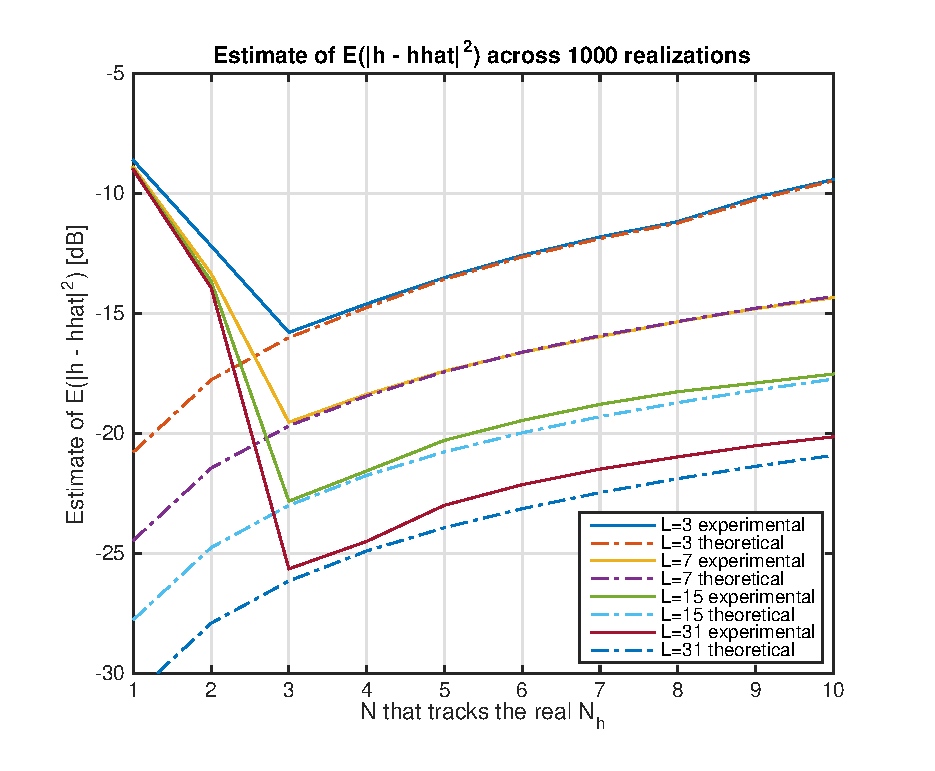
\includegraphics[width=0.75\textwidth]{p02_comparetheoreticaldeltah}
	\caption{Experimental estimation error $E[||\mathbf{\Delta h}||^2]$ with different values of $L$ and $N$, compared with its theoretical value.}
    \label{fig:p02_comparetheoreticaldeltah}
\end{figure}


\begin{thebibliography}{10}

\bibitem{bc}
Benvenuto, Cherubini, Algorithms for Communications Systems and their Applications, Wiley, 2004

\bibitem{anachugg}
Anastasopolous, Chugg, An efficient method for simulation of frequency selective isotropic Rayleigh fading, IEEE 47th Vehicular Technology Conference, vol 3, pages 2084 - 2088, 1997

\end{thebibliography}

\end{document}
